\documentclass[12pt, letterpaper]{report}
\usepackage[spanish, es-tabla]{babel}% coloca tabla en lugar de cudro en las tablas e idioma español.
% Dimensiones y márgenes---------------------------------------------

\usepackage[total={18cm,21cm},top=4cm, left=2cm, right = 3 cm]{geometry}
\usepackage[scaled]{helvet}
\renewcommand*\familydefault{\sfdefault} 
%\usepackage[T1]{fontenc}
% Otros paquetes -----------------------------------------------------
\usepackage{mathpazo} %fuente palatino
\usepackage{graphicx} %paquete para gáficos
%\usepackage[usenames]{color}	%paquete para colores
\usepackage{pstricks}	
\usepackage[utf8]{inputenc}
%\usepackage[shortlabels]{enumitem}
% Referencias para graficos
\usepackage{graphicx} % gráficos
\usepackage{subfigure} % subgráficos
% Referencias - ligas
\usepackage[hyphens]{url}
\usepackage[breaklinks,colorlinks=true,linkcolor=black, citecolor=red, urlcolor=blue]{hyperref}
%Paquetes adicionales de símbolos matemáticos
\usepackage{amsmath,amssymb,cancel}% funciones matematicas ,amsfonts ,latexsym
%Comandos ---------------------------------------------------------
\usepackage{fix-cm} % Allows increasing the font size of specific fonts beyond 
\usepackage{colortbl} % Comandos personales - especiales
\usepackage{ multirow, array} % para las tablas
\usepackage{float} % para usar [H]
\usepackage{longtable} % para tablas largas
%\pagestyle{empty}
\usepackage{booktabs}
\usepackage{fancyhdr}
\usepackage{rotating}% paquete para rotar
\usepackage{multicol}
\usepackage{verbatim}
\usepackage{sidecap}
\usepackage{wrapfig}
%\usepackage{html,makeidx}
%\usepackage{cite}
%\pagestyle{myheadings}% estilo de pagina propio
%\markright{\rightmark} %\usepackage{fancyhdr}% para los estilos de encabezado y pie de pagina
\pagestyle{fancy}% estilo de pagina
%\fancyfoot[LE,RO]{\thepage}
% cabecera y pie
\lhead{Página \thepage } % texto izquierda de la cabecera
%\chead{TEXTO} % texto centro de la cabecera
%\rhead{\thepage} % número de página a la derecha
\lfoot{} % texto izquierda del pie
%\cfoot{\includegraphics[width = 1cm]{universidad.png} } % imagen centro del pie
%\rfoot{ \textit{Maestria en Ingenieria con Énfasis en Ing. Eléctrica}} % texto derecha del pie
%\renewcommand{\headrulewidth}{0.4pt} % grosor de la línea de la cabecera
%\renewcommand{\footrulewidth}{0.4pt} % grosor de la línea del pie
%LaTeX default specifications
%more content to this template
\usepackage{acronym} %definiciones de acronimos
\definecolor{grey}{rgb}{0.9,0.9,0.9} % Color of the box surrounding the title - these values can be changed to give the box a different color	





\begin{document}
\title{tesis}
\author{Alejandro Palacios Carabali.}
\date{2017}
%\tableofcontents
%----------------------------------------------------------------------------------------
%	TITLE SECTION
%---------------------------------------------------------
\thispagestyle{empty}% pagina no numerada	
\colorbox{grey}{
	\parbox[t]{1.0\linewidth}{
		\centering \fontsize{20pt}{30pt}\selectfont % The first argument for fontsize is the font size of the text and the second is the line spacing - you may need to play with these for your particular title
		\vspace*{0.7cm} % Space between the start of the title and the top of the grey box
		
		\hfill \textbf{ ESTADO DEL ARTE}\\ 
		\hfill \textbf{SOBRE }\\
		\hfill \textbf{ESTRATEGIAS }\\
		\hfill \textbf{PARA LA REGULACIÓN DE} \\
		\hfill \textbf{VOLTAJE EN REDES DE } \\ 
		\hfill \textbf{DISTRIBUCIÓN ELÉCTRICA } \\ 
		\hfill \textbf{CON ALTO GRADO DE}\\
		\hfill \textbf{GENERACIÓN }\\
		\hfill \textbf{DISTRIBUIDA }\\
		\hfill \textbf{RENOVABLE }\\
		\par
		
		\vspace*{0.7cm} % Space between the end of the title and the bottom of the grey box
	}
}

%----------------------------------------------------------------------------------------

\vfill % Space between the title box and author information

%----------------------------------------------------------------------------------------
%	AUTHOR NAME AND INFORMATION SECTION
%----------------------------------------------------------------------------------------

{\centering \large 
\hfill Alejandro Palacios \\
\hfill Universidad del Valle \\
\hfill Escuela de Ingeniería Eléctrica y Electrónica \\
\hfill Directores:\\
\hfill Diego Fernando Echeverry\\
\hfill Sandra Milena Londoño\\

}
%{1pt}} % Horizotal line, thickness changed here

%----------------------------------------------------------------------------------------
\sloppy

\setlength{\parindent}{0cm}


%%%%%%%%%%%%%%%%%%%%%%%%%%%%%%%%%%%%%%%%%%
%%%%%%%  TABLA DE CONTENIDO %%%%%%%%%%%%%%
%%%%%%%%%%%%%%%%%%%%%%%%%%%%%%%%%%%%%%%%%%

\tableofcontents % indice de contenidos

\cleardoublepage
\addcontentsline{toc}{chapter}{Lista de figuras} % para que aparezca en el indice de contenidos
\listoffigures % indice de figuras

\cleardoublepage
\addcontentsline{toc}{chapter}{Lista de tablas} % para que aparezca en el indice de contenidos
\listoftables % indice de tablas
%%%%%%%%%%%%%%%%%%%%%%%%%%%%%%%%%%%%%%%%%
%%
%%  Definicones de Acronimos
%%
%%
%%


\chapter*{Lista de Acrónimos}

\addcontentsline{loc}{chapter}{Lista de Acrónimos}

\begin{acronym}
	\begin{multicols}{2}
    \acro{ADA}{Advanced Distribution Automation}
    \acro{AVC}{Automatic Voltage Control}
	\acro{DG}{Distributed Generation}
    \acro{DS}{Distribution System}
    \acro{EES}{Energy Storage System}
    \acro{EPS}{Electrical Power System}
    \acro{FL}{Fuzzy Logic}
    \acro{GA}{Genetic Algoritm}
    \acro{LDC}{Load Drop Control}
    \acro{LV}{Low Voltage}
    \acro{MR}{Micro Redes}
    \acro{OR}{Operador de Red}
    \acro{RES}{Renaovable Energy Sources}
    \acro{SG}{Smart Grid}
    \acro{ST}{Smart Transformer}
    \acro{SVC}{Static Var Compensator}
    \acro{SVR}{Static Voltage Regulador}
    \acro{OLTC}{On Load Tap Changer}    
    \acro{PV}{Photovoltaic Generator}
    \acro{PQ}{Power Quality}
    \acro{UF}{usuarios finales}
    \end{multicols}
    
\end{acronym}

%%%%%%%%%%%%%%%%%%%%%%%%%%%%%%%%%%%%%%%%%
\chapter*{INTRODUCCIÓN}
Los \textit{sistemas de distribución eléctrica} (\ac{DS} ) son la ultima etapa en el transporte de energía,  desde los generadores hasta los \ac{UF} dentro del sistema eléctrico de potencia (\ac{EPS}) \cite{basso2004ieee}. La electricidad transportada a través de los \ac{DS} en las dos décadas anteriores se ha caracterizado por provenir en mayor grado de fuentes hidráulicas, nucleares y  fósiles ( como carbón, petroleo, gas, etc) \cite{Bacha2015}. Estas ultimas fuentes de energía, al ser empleadas tanto para la generación eléctrica como en es sector del transporte \cite{Bahmanifirouzi2012}, han traído como consecuencia un incremento del calentamiento global a raíz  de los gases de efecto invernadero que se liberan en  su proceso de combustión  \cite{Hauck2017}.\\\\
Como respuesta a esta problemática en los años recientes se ha dado  paso al incremento de la generación a pequeña  escala instalada dentro del \ac{DS} conocida como generación distribuida  \ac{DG} ya sea de carácter renovable   \ac{RES} como la fotovoltaica, solar térmica, eólica, biomasa y micro turbinas hidráulicas  \cite{Calderaro2014} o no renovable. \\\\
Esta nueva red que contiene fuentes de \ac{DG}, en la cual aparecen intercambios de potencia bi direccionales  e implementa funcionalidades inteligentes,  haciendo uso  o no de una una infraestructura de telecomunicaciones, para lograr la adaptabilidad se conoce como \ac{SG} \cite{Bhatt2014}.\\\\ 
Dado este contexto la \ac{DG} puede funcionar  en conjunto con  algunas cargas para suplir su demanda, ya sea de manera total o  parcial. Cuando ocurre de manera total se da lugar a  un muevo escenario dentro de las \ac{SG}  conocido como \ac{MR} \cite{Pegueroles-Queralt2012}, las cuales son redes eléctricas en pequeña escala  con niveles de tensión de distribución ($\leq$ 20 kV)  y potencias menores a 1MW ( por lo general) \cite{Bacha2015}, pudiendo operar de manera autónoma o  conectada al \ac{DS}. Estas \ac{MR} suelen también  tener elementos de almacenamiento de energía conocidos como \ac{EES} \cite{Colak2015} con el fin de lograr funcionalidades autonomía, estabilidad  y calidad de energía.  \cite{Babacan2017} \cite{Pegueroles-Queralt2012}.\\\\ 
Tanto en la operación de las  \ac{MR} como dentro de los \ac{DS}, estos \ac{RES}  al inyectar potencia  al \ac{DS}  generan a través de  él  una elevación de tensión \cite{GSGF2015} como lo muestra la figura \ref{fig:ejemplo_control_de_tension}; esta elevación de tensión es en proporción a la potencia inyectada por la \ac{DG} , en el caso  de la figura \ref{fig:ejemplo_control_de_tension} con generadores tipo fotovoltaicos  (\ac{PV}). Esta situación es contraria al caso clásico en donde no hay \ac{DG} ( consumer ) y la tensión va disminuyendo desde la subestación eléctrica del OR hasta las instalaciones del usuario final \ac{UF}. Esta desviación de tensión  dependerá principalmente de la magnitud de los flujos de potencia bidireccionales \cite{Koutsoukis2017}, la ubicación de la \ac{DG} \cite{Othman2016a}, la topologia de la red y las impedancias del \ac{DS} .\\\\
Sumado a esto se debe tener en cuenta que algunas de las \ac{DG} como la \ac{PV} y la eólica,tienen un carácter  intermitente y su generación de energía  es afectado por  las condiciones ambientales (principalmente climáticas) \cite{Mahmud2016}. Esto causa problemas de estabilidad, confiabilidad, aumento en las perdidas y mala \textit{calidad de energía} \cite{Karanki2014}\cite{DinakaraPrasadReddy2017}.\\\\

 \begin{figure}[H]
 	\centering
 	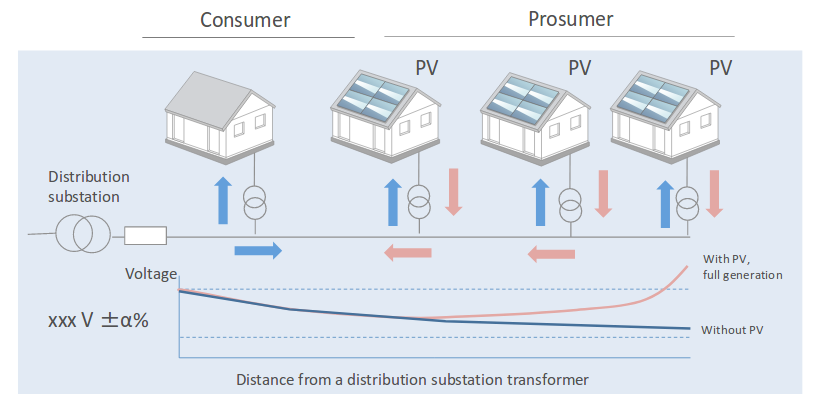
\includegraphics[width=0.7\linewidth]{imagenes/ejemplo_control_de_tension}
 	\caption{Concepto de incremento de tensión en los sistemas de distribución \cite{GSGF2015} }
 	\label{fig:ejemplo_control_de_tension}
 \end{figure}
 
Entre los parámetros más importantes de  calidad de la energía se encuentra el \textit{nivel de tensión}. Cuando el nivel de tensión se encuentra fuera del \textit{rango permitido} ocasiona daños en los las cargas principalmente las que tienen un alto componente electrónico \cite{baggini2008handbook}.\\\\
Para dar solución a esta problemática los operadores de red OR clasicamente han implementado esquemas basados en cambiadores de taps en los transformadores (\ac{OLTC})  y bancos de condensadores \cite{Acha2002a}\cite{Bisanovic2014}, comandados ya sea de forma manual o automática para responder a los cambios en la tensión provocados por la demanda \cite{Gubina2001}. En un escenario con \ac{DG} se deben replantear estos esquemas de control de tensión \cite{Yadav2014} que le permitan a los \ac{OR} mantener el nivel de tensión en los rangos permitidos. Por tanto este trabajo se realizara una revisión  de  las soluciones mas destacadas  para realizar el control de la tensión en un \ac{DS} cuando hay presencia de \ac{DG} de tipo \ac{RES}. \\\\
La metodología de investigación es del tipo \textit{correlacional}, está parte  de realizar un estudio \emph{descriptivo} del fenómeno,  explorando sus contenidos  y  evaluando  sus tópicos de manera analítica. Una vez obtenido  esto  se pasa a un trabajo comparativo  en el cual se establecen las    \textit{relaciones} que describan de modo cualitativo y/o cuantitativo  el tema en estudio . La técnica a emplear en este trabajo sera el \textit{análisis documental} que buscan describir y representar los documentos de forma unificada sistemática para facilitar su recuperación.\\
En el capitulo  \ref{cap:teorico} se hace referencia  a los principales conceptos necesarios para abordar la investigación, el capitulo \ref{cap:clasificacion} se realiza una caracterización de las  fuentes bibliográficas a partir de unos \textit{criterios documentales} o temáticas de investigación,  el capitulo \ref{cap:documental}  se realiza un análisis de las temáticas escogidas como \textit{criterios de análisis }, para finalmente en capitulo  realizar  la perspectiva trazada por el autor sobre este tema.

\chapter{MARCO TEÓRICO}
\label{cap:teorico}
\section{CAÍDA DE TENSIÓN CON GENERACIÓN DISTRIBUIDA}
Con el crecimiento de la \ac{DG} \cite{Cao2016} en los \ac{DS} se ha dado lugar a la aparición de flujos de potencia inversos ( es decir desde la carga hacia el \ac{DS}) lo cual, acompañado por los altos valores en la relación R/X (resistencia reactancia) que caracteriza principalmente a los circuitos de \ac{LV}, dan lugar a la aparición de sobre tensiones en los nodos del  \ac{DS} \cite{su2009comparative}\cite{Tang2017}.\\

\begin{wrapfigure}{O}{8 cm}
	\begin{center}
		\caption{Diagrama unifilar de una red simplificada}
		\label{fig:dos_nodos}
		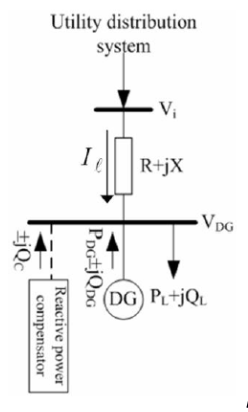
\includegraphics[width=0.6\linewidth]{imagenes/cap_1/dos_nodos}
	\end{center}	
\end{wrapfigure}

Para ilustrar este fenómeno se parte  del diagrama unifilar de la figura \ref{fig:dos_nodos} en el que se representan las características básicas de un sistema de potencia con \ac{DG}. Este esta conformado por la carga que demanda una potencia $P_{L}+jQ_{L}$, la DG que genera o absorbe una potencia $P_{DG}\pm jQ_{DG}$,  la compensación reactiva que inyecta o absorbe una potencia $\pm jQ_{C}$, la impedancia de linea $R+jX$,  los nodos $V_{i} $ de entrada y $V_{DG}$ en la carga y el equivalente de red del sistema.\\

De acuerdo a la definición de potencia compleja se tiene la siguiente expresión \cite{Akagi2017}:\\

\begin{equation}
\label{equ:comp}
P + jQ = V_{DG} \cdot I_{l}^{*}
\end{equation}

De la ecuación \ref{equ:comp}  se puede obtener  la corriente de línea en función de la potencia activa y reactiva :

\begin{equation}
I_{l}= \dfrac{P + jQ}{\overrightarrow{V_{DG}^{*}}}
\label{eq:corriente}
\end{equation}

Aplicando el la ley de \textit{ Kirchoff } de tensiones en el nono  $V_{GD}$, este  puede ser expresado como:\\\\
\begin{equation}
\label{equ:volt_gd}
\overrightarrow{V_{DG}}= \overrightarrow{V_{i}} + I_{l}(R + X_{L})
\end{equation}

Remplazando $ I_{l} $ de  la ecuación \ref{eq:corriente} en la ecuación  \ref{equ:volt_gd} se tiene:

\[\overrightarrow{V_{DG}}= \overrightarrow{V_{i}} + \dfrac{P + jQ}{\overrightarrow{V_{DG}^{*}}}(R + X_{L})\]

\begin{equation}
\overrightarrow{V_{DG}}= \overrightarrow{V_{i}} + \dfrac{RP + X_{l}Q}{\overrightarrow{V_{DG}^{*}}} + j\dfrac{RP - X_{l}Q }{\overrightarrow{V_{DG}^{*}}}
\end{equation}

Cuando el ángulo entre los fasores de tensión  $V_{DG}$  y $V_{l}$ es pequeño, es decir cuando la potencia activa entregada por el DS tiende a cero \cite{Akagi2017} (  esto puede darse porque no hay demanda de energía o la $DG$ abastece la demanda de la carga en una condición de auto consumo de los usuarios o de la micro red), y si además de ello se considera el voltaje en el nodo $V_{DG}$ como referencia fasorial (ángulo 0) la caída de tensión en la línea puede ser escrita como:\\\\
\begin{equation}
\Delta\ V \cong V_{DG} - V_{i}\cong \dfrac{RP - X_{l}Q }{V_{DG}}
\label{eq:delta} 
\end{equation}
Donde, $\Delta V$ es la caída de tensión a través del alimentador. Si también asumimos que la tensión en el nodo  $V_{DG}$  es la tensión base, entonces podemos reescribir la ecuación \ref{eq:delta} como:\\\\
\begin{equation}
\Delta\ V \cong V_{DG} - V_{i}\cong RP - X_{l}Q 
\label{eq:delta1} 
\end{equation}
Donde $P=(P_{DG}-P_{L})$  y  $ Q = (\pm Q_{DG} \pm Q_{c} - Q_{L})$.\\\\
De este modo la ecuación \ref{eq:delta1} puede ser reescrita así:

\begin{equation}
V_{DG} \cong V_{i} + R (P_{DG} - P_{L}) + X(\pm Q_{DG} \pm Q_{c} - Q_{L})
\label{eq:voltajeds}
\end{equation}
De este modo  de la ecuación \ref{eq:voltajeds} se puede determinar  el nivel máximo de generación que puede  albergar un circuito.\\\\
Para tal caso se plantean dos escenarios críticos en los cuales se presentan las máximas desviaciones de tensión \cite{Elkhatib2011a}:\\\\

\begin{table}[h]
	\centering
	\caption{Escenarios de tensión }
	\label{tab:escenarios_v}
	\vspace{0.5 cm}
\begin{tabular}{|c|c|c|}
    \hline 
    Caso 	& Carga 	& Generación \\\hline
    1 		& Mínima	& Máxima \\\hline
    2		& Máxima	& Mínima \\
    \hline
\end{tabular}
\end{table}

\subsection{Caso crítico carga mínima  y máxima generación }
Se considera este primer escenario en el cual la demanda de la carga es mínima, por ejemplo  para una carga residencial típica  esto es  en las horas de la madrugada. La otra condición de máxima generación se presenta por ejemplo para fuentes fotovoltaicas  en el medio día,  con lo cual se podría tener que para un caso típico de carga residencial con generación fotovoltaica esta condición se alcanzaría en medio día.\\\\
Esto se puede  cuantificar a partir de la ecuación \ref{eq:voltajeds} se tenga un factor de potencia igual a uno  en el nodo  $V_{DG}$, entonces se puede deducir que la máxima tensión en este nodo se obtiene cuando hay la mínima carga ($P_{L} = 0$ , $Q_{L} = 0$ )  y la generación máxima ($P_{G} = P_{GMAX}$). En estas condiciones el OR puede operar incluso sin que exista generación distribuida. la tensión en el nodo $V_{DG}$, queda determinado entonces por la ecuación \ref{eq:voltajeds} así \cite{strbac2002integration} :\\\\
\begin{equation}
V_{DG} = V_{i} + P_{GMAX}
\label{eq:vgmax}
\end{equation}


\begin{tabular}{l c r}
    & &\\
    Donde:& & \\
    & &\\
    & $P_{GMAX}$ & Es la potencia máxima permisible en el \ac{DS}.\\
    & &\\
    & &\\
\end{tabular}\\\\
En estas condiciones la potencia máxima permisible en el sistema es :\\\\
\begin{equation}
P_{GMAX} \leq \frac{V_{DGMAX} - V_{i}}{R}
\label{eq:pgmax}
\end{equation}
\begin{tabular}{l c r}
    & &\\
    Donde:& & \\
    & &\\
    & $V_{DGMAX}$ & Es la tensión máxima permisible en el \ac{DS}.\\
    & &\\
    & &\\
\end{tabular}\\\\
Se puede notar en la ecuación \ref{eq:pgmax} la potencia máxima generada es función de la resistencia de línea, de modo tal que la resistencia de la linea ( que depende del calibre del conductor y la longitud ) determina la máxima potencia que puede ser inyectada al sistema.\\
\subsection{Caso critico máxima carga y mínima generación }
Se considera este segundo escenario en el cual la demanda es alta , por ejemplo  para una carga residencial típica  esto es  en el inicio de la noche o iniciando la mañana y ademas la generación producida por los diferentes \ac{DS} es baja.\\\\
Considerando igualmente un factor de potencia unitario por tanto la ecuación \ref{eq:voltajeds} puede ser  escrita para este caso así:

\[V_{DG} = V_{i} - RP_{Lmax}\]

O

\[P_{Lmax} = \dfrac{V_{i} - V_{DG }}{R}\]

Consideremos ahora que $V_{DGmin}$ es el mínimo voltaje permisible en el \ac{DS}. Por tanto para mantener el voltaje bajo los limites permisibles  se debe cumplir que:

\[P_{Lmax} \leq \dfrac{V_{i} - V_{DGmin}}{R}\]

\subsection{Dependencia del factor R/X}
Otro indicador importante al momento de establecer el control de tensión es el factor $ R/X$ del equivalente de red, donde $R$  y $X$ son respectivamente la resistencia y la reactancia  \textit{Thevenin} del \ac{DS} en el nodo $V_{GD}$.    Para \textit{valores bajos} del parámetro $R/X$ ( es decir donde el equivalente de red es principalmente reactivo ) la potencia activa tiene muy poca  influencia en los perfiles de tensión, mientras conforme el parámetro $R/X$ crece, el efecto de la potencia activa sobre las tensiones es mas determinante. Dicho de otro modo, en \textit{media tensión } y baja tensión la inyección de potencia activa por parte de la GD provoca aumentos de la tensión en el PCC.\\\\
De algún modo este efecto de la potencia activa en los niveles de tensión debe ser mantener la tensión en el punto de nominal compensado mediante la absorción de potencia reactiva para devolver los niveles de tensión a su condición de diseño.\\\\
La potencia reactiva necesaria para mantener la tensión en el nodo $ V_{DG}$ ( figura \ref{fig:dos_nodos}), en cuanto mayor es el parámetro $R/X$ es necesario absorber una mayor cantidad de potencia reactiva  para mantener la tensión en el PCC. Nótese que en redes de media tensión ($R/X$ alrededor de la unidad) la cantidad de  reactiva necesaria para compensar el efecto de la potencia activa es 2 a 1. \cite{trebolle2012control}.

\section{ELEMENTOS DE CONTROL DE TENSIÓN}

 \subsection{Cambiador de Taps bajo Carga}
El cambiador de tomas bajo carga \ac{OLTC} es un equipo  cuya función es conmutar las conexiones de derivación del devanado de un transformador ( puede estar el primario o en el secundario) en estado energizado o en carga, estos son diseñados bajo los criterios de la norma IEC 60214-1 \cite{IEC60214}.
El equipo encargado de del operar el \ac{OLTC} es conocido como \ac{AVC}, el cual conmuta las sus derivaciones del transformador de acuerdo a la desviación que se presente con respecto al la tensión de referencia o tensión objetivo, esto se puede ilustrar en la figura \ref{fig:esqusema_LDC} \cite{Sarimuthu2016}. Este control debe asegurarse que el voltaje se encentre siempre por encima del nivel mínimo de tensión el cual decrece a lo largo del circuito \cite{Sarimuthu2016} para el caso de un circuito radial sin DG. Las  mediciones realizadas en la figura \ref{fig:esqusema_LDC} son usadas para calcular la caída de tensión en el nodo remoto, esta técnica es conocida como \ac{LDC}.\\\\

\begin{SCfigure}[\sidecaptionrelwidth][!hb]
\centering
\caption{Esquema de controlador para OLTC con LDC \cite{Sarimuthu2016}}
\label{fig:esqusema_LDC}
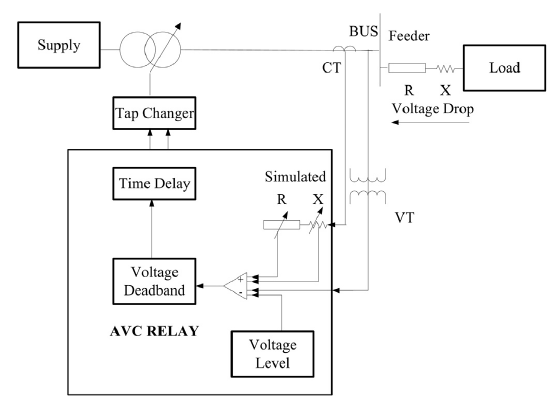
\includegraphics[width=8cm]{imagenes/cap_2/LDC}
\end{SCfigure}


\subsection{Regulador de Tensión}
Otro dispositivo similar al este es el \ac{SVR} el cual consiste en un auto transformador con un cambiador de taps  bajo carga \cite{Vkdulqj}. Por lo general son diseñados para regular la tensión en rangos de $\pm 10 \%$ de la tensión nominal en 32 pasos \cite{kersting2009modeling} \cite{farag2012incorporating}. La norma ANSI/IEEE C57.15 establece dos rangos de tensión para la operación, uno en estado normal ( rango A) y otro en estado de contingencia ( rango B).

\begin{figure}[H]
	
\centering
\subfigure[ Diagrama interno del \ac{SVR} \cite{Oshiro2011a}]{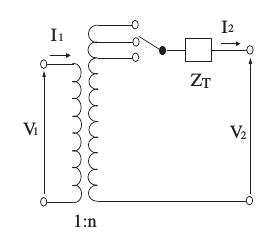
\includegraphics[width=5cm]{imagenes/cap_2/regulador}}
\hspace{5mm}
\hfill
\subfigure[Control de caida de tensión \ac{LDC} basado en \ac{SVR} \cite{Vkdulqj} \label{fig:ldc_svr}]{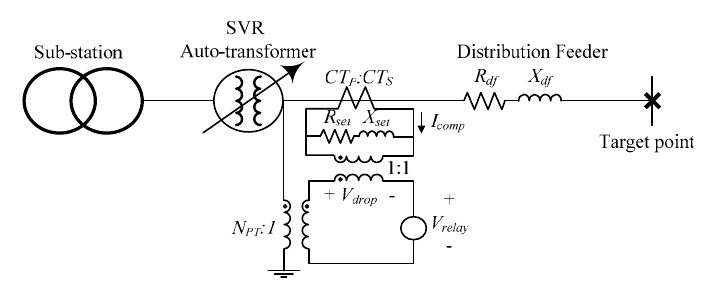
\includegraphics[width=10cm]{imagenes/cap_2/LDC_SVR}}
\caption{Esquema del regulador de tensión}
\label{fig:regulador}

\end{figure}

La posición del \ac{SVR} es  controlada  mediante el esquema de \ac{LDC} similar mente al \ac{OLTC}. Dado esto como se muestra en la figura \ref{fig:ldc_svr} el controlador  debe de conocer la impedancia del sistema ( \textit{distribution fider}) para ajustar la tensión en el nodo remoto ( \textit{target point}) \cite{Vkdulqj}.
\subsection{Compensador de Var Sincrono}

\subsection{Generadores Fotovoltaicos }

Los generadores fotovoltaicos \ac{PV} se caracterizan por inyectar corriente 

\begin{figure}[h]
\centering
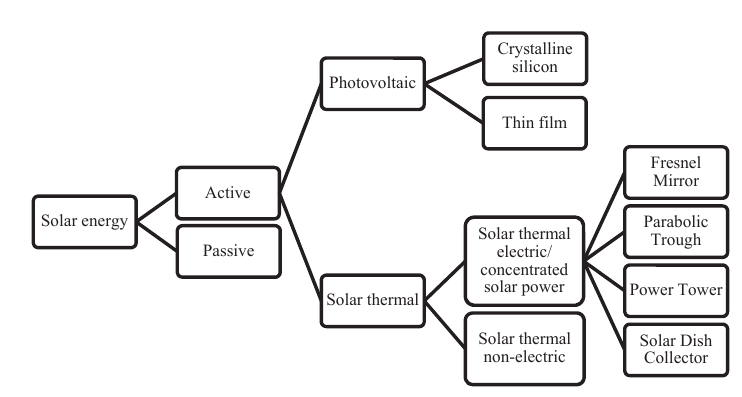
\includegraphics[width=0.7\linewidth]{imagenes/cap_1/sistemas_solares}
\caption{Variedad de fuentes fotovoltaicas}
\label{fig:sistemas_solares}
\end{figure}

\subsection{Transformador inteligente (Small Transformer)}
El transformador inteligente o \ac{ST} \cite{Colak2015}


\subsection{Convertidores de Potencia}

\subsubsection{Inversores}

Existen dos métodos de control básicos para los inversores: control en cascada y
control del estado-espacio (\textit{state-space}) \cite{Bacha2015}. La figura \ref{fig:tensionpv} muestra el esquema de control básico de un inversor modular monofásico, que también se puede utilizar  para un inversor trifásico (empleando tres módulos). Los bloques verdes muestran el hardware de la electrónica de potencia, los bloques azules muestran los dispositivos de medición de corrientes y tensiones, y los bloques rojos muestran las partes del controlador en cascada.
Si el interruptor está en la posición 1, el inversor funciona como una fuente de corriente para alimentación de red. El MPPT (maximum
power point tracking) calcula el punto de ajuste para la tensión continua el cual alimenta a un control  proporcional-integral . Dado que la salida del controlador de voltaje de corriente continua es un punto de consigna de CC, para el valor RMS de la corriente alterna, se debe multiplicar con la tensión de corriente alterna normalizada y filtrada para obtener un punto de consigna de corriente alterna.
Si el interruptor está en la posición 2, el inversor funciona como una fuente de voltaje para el modo de isla. El punto de ajuste para la tensión de alterna se calcula con el microcontrolador o procesador de señal digital. Un controlador de compensación de DC especial controla el desplazamiento de CC de la tensión de CA a cero. \cite{Burger2001a}, que controla el valor RMS de la tensión alterna. Si varios inversores están conectados en paralelo en una microgrid isla, pueden usarse controladores adicionales para calcular los puntos de ajuste de la tensión y la frecuencia de CA \cite{Bacha2015} .
\begin{figure}[h]
\centering
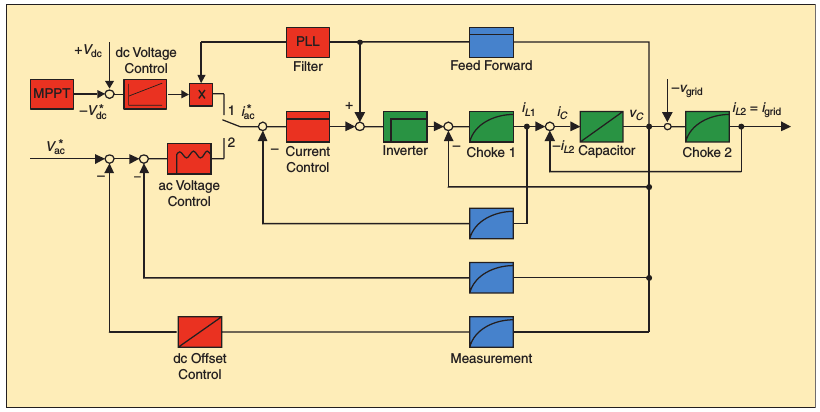
\includegraphics[width=1\linewidth]{imagenes/tension_pv}
\caption{Esquema de control básico de un inversor conectado a una red monofásica (switch en posición 1) y la operación en modo isla (switch en posición 2). Las características del inversor aparecen en color verde , los elementos de medida en color azul, y los controladores en cascada en color rojo.\cite{Bacha2015}}
\label{fig:tensionpv}
\end{figure}

\subsection{Conversores back to back}

\begin{comment}

%reactive power control of capacitor bank using changes in
%reactance of connected reactor vary their demand for reactive power
%voltage regulation, power-factor correction and reactive power compensation
%voltage profile and reduction of power losses.
% loads that vary their demand for reactive power 
% the variation in demand for reactive powercauses variation in the voltage at the supply point that can interfere with the efficient operation of supply network
%resonance problems is to install large capacitor banks at the main bus.
% In these applications mechanically switched capacitor banks  are the most economical reactive power compensation resource
%no effect on the short-circuit power and low-cost, but low-speed solution for voltage control
%  capacitor banks as smooth output or output in very small blocks.
% minimal number of switches and become very rational
%  selection of the optimal size and allocation of capacitor banks.
% unbalanced distribution systems is presented. This method dynamically coordinates between voltage and reactive power generation and consumption to keep the bus voltages close to their nominal value
% The static VAr compensator  thyristor-switched capacitors (TSC),  thyristor-controlled reactors (TCR),


%incorporating voltage dependency of loads in the process of phase-balancing.
\cite{Singh2016}

\cite{Oshiro2011a}

\label{cap_planeacion}
\cite{Idlbi2013}
\end{comment}
\section{MÉTODOS DE OPTIMIZACIÓN}
\subsection{Algoritmos Genéticos}


\subsection{Lógica Difusa}

\subsection{Agentes Inteligentes}

\section{ANÁLISIS FINANCIERO}

\chapter{CLASIFICACIÓN DE MATERIAL BIBLIOGRÁFICO}
En este capitulo se muestra el proceso de recopilación documental realizado a  la muestra. Para comenzar se definieron los \textit{criterios de búsqueda}, los cuales constituyen los parámetros básicos para asignar al gestor documental la información necesaria para acotar el universo de documentos obtenidos. De este modo se establecieron los siguientes criterios:\\

\begin{itemize}
    \item \textit{Palabra clave: \textit{Control voltage}}
    \item \textit{Palabra clave: \textit{Distributed generation}}
    \item \textit{Area : Ingeniería}
    \item \textit{Periódo: 2013 -2017}
\end{itemize}

En estos criterios las  palabras claves se emplean dentro de la búsqueda para optimizar la pertinencia de los contenidos la temática  de estudio. Para identificar la muestra documental se empleo la herramienta informática SCOPUS, de la cual  se obtuvieron un total de 399 documentos indexados. Para garantizar  la \textit{diversidad} de la muestra, se establecieron los siguientes valores como \textit{mínimos de referencia}.

\begin{itemize}
	\item Se deben incluir mínimo el 50\% de la bibliografia encontrada para los 5  paises mar relevantes.
	\item Se deben incluir mínimo los el 50\% de la bibliografia de los tres autores más relevantes.
\end{itemize}

De los resultados arrojados por la herramienta SCOPUS los tres principales autores y los cinco países mas destacados son los  mostrados en la tabla:\\

\begin{table}
    \caption{Aplicación de los criterios de búsqueda}
    \label{tab:criterios_busqueda }
\begin{tabular}{|l| m{3 cm}| m{3 cm}| m{3 cm} | m{2.8cm} |}
    \hline
    CRITERIO & NOMBRE &  ARTÍCULOS & PORCENTAJE & MÍNIMO DE ARTÍCULOS \\\hline
    \multirow{3}{4cm}{Autor} & Muttaqi, K.M. & 7 & 50 \% & 4\\\cline{2-5}
    & Pota, H.R.
     & 7 &50 \% & 4\\\cline{2-5}
    & Hamzeh, M.
      & 5 & 50 \% & 3\\\hline
    \multirow{5}{4 cm}{Pais} & China & 71 &50 \% & 36 \\\cline{2-5}
    & Estados Unidos & 40 &50 \% & 20 \\\cline{2-5}
    & india & 36 &50 \% & 18\\\cline{2-5}
    & Iran & 29 &50 \% & 14 \\\cline{2-5}
    & Canada & 24 &50 \% & 12\\\hline

   
\end{tabular} 
\end{table}



\chapter{ANÁLISIS DOCUMENTAL}
\label{cap:documental}

Este  análisis  consiste en evaluar el aporte de las diferentes fuentes bibliográficas a cada una de las temáticas abordadas  como \textit{criterios de análisis}. Dentro de este trabajo de investigación estos criterios de análisis fueron escogidos por el autor de acuerdo a la pertinencia que tienen los mismos dentro del marco conceptual referente a las \ac{SG} enfatizándose dentro de esta en los aspectos de  automatización de la red \ac{ADA} y la calidad de la energía \ac{PQ}.\\\\ 

Los criterios de análisis son entonces los siguientes:

\begin{enumerate}
    \item Micro redes.
    \item Planeamiento de la red.
    \item Impacto de las fuentes fotovoltaicas.
    \item Impacto de las fuentes eólicas.
    \item Flujo de potencia activa y reactiva.
    \item Control local  o centralizado.
    \item Optimización de la capacidad de alojamiento.
    \item Análisis técnico - económico.
    \item Impacto del almacenamiento de energía.
    \item Control de tensión en redes en DC.
\end{enumerate}

\section{MICRO REDES}
\section{PLANEAMIENTO DE LA RED}

\section{IMPACTO DE LAS REDES FOTOVOLTAICAS}

En \cite{Oshiro2011a} se plantea un control de tensión centralizado,  el cual responde con  cambios en la potencia reactiva inyectada por cada inversor tras  ocurrir cambios condiciones climatologías ( que afectan la cantidad de $kW/m^{2}$), la cantidad de potencia reactiva es calculada resolviendo el problema de optimización  basado en algoritmos genéticos \ac{GA} el cual a su vez controla los \ac{SVR}  y los \ac{SVC} que se encuentran el el sistema. 
En \cite{Shalwala2011a} se realiza un control de centralizado  de tensión sobre un área residencial con alto grado de penetración de sistemas \ac{PV} basado en \ac{FL}. Tiene como parámetros  de entrada el área de las edificaciones, las curvas de radiación solar para controlar los \ac{OLTC}.  

\section{IMPACTO DE LAS REDES EÓLICAS}


\section{FLUJO DE POTENCIA ACTIVA Y REACTIVA}

%\section{RE CONEXIÓN DE CIRCUITOS DE DISTRIBUCIÓN}
%\label{cap:clasificacion}
%En \cite{Cao2016} se propone el uso de dispositivos electrónicos para transferir potencia reactiva en las fronteras de los circuitos del \ac{DS}, esto lo realiza mediante conversores back to back. Se noto que se mejora el des balance de la red a su vez que se minimizan las perdidas, logrando mayor efectividad cuando se usa en combinación con la DG y la re configuración de circuitos manteniendo la tensión en los niveles esperados.\\

\section{CONTROL LOCAL O CENTRALIZADO}
En \cite{Efkarpidis2016} se propone un sistema híbrido para el control de tensión en LV empleando de manera combinada \ac{OLTC} y control de potencia activa y reactiva mediante inversores monifásicos, en tal caso el \ac{OLTC} resulta ser el método mas efectivo para controlar los percentiles de la tensión.En \cite{Colak2015} plantea el uso se \ac{ST} para controlar la tensión y la transferencia de potencia activa de modo instantáneo en las zonas donde este alimenta el \ac{DS}  que contienen alto grado de \ac{PV}. En \cite{Calderaro2014} se presenta un método de control basado en redes neuronales  capaz de controlar la tensión el los nodos de forma autónoma maximizando la potencia activa inyectada por los \ac{DS}. El controlador usa solamente la modulación en potencia activa si la modulación  de potencia reactiva no es suficiente, este método es probado tanto en fuentes fotovoltaicas  como en eólicas.\\  

En el entorno de las \ac{SG}, algunos de los  \ac{DG} son despachados de modo central empleando apara ello diversas estrategias de control , mientras que por otro lado las \ac{DG} no despachadas como plantas solares y eólicas son controladas mediante un rango optimo predefinido de tensión \cite{Vandoorn2013} \cite{colak2015survey}.
En \cite{Oshiro2011a} se plantea un esquema de control centralizado mediante \ac{GA}  en el que se consideran los inversores SVC,  en \cite{Shalwala2011a} se considera un control \ac{FL} que controla los \ac{OLTC}  con alta penetración de sistemas \ac{PV}.

\section{OPTIMIZACIÓN DE LA CAPACIDAD DE ALOJAMIENTO (HOSTING CAPACITY)}	
La capacidad de alojamiento (HC \textit{hosting Capacity}) consiste en cuantificar el impacto que tendrá un incremento de la DG \cite{Bollen2008}.\\
En \cite{Caldon2015a} se plantea una estrategia de control de tensión sobre los DER ubicados dentro  de usuarios finales en el contexto de madurez de las \textit{smart grid}, lo que permite emplear la infraestructura de comunicación, distribuyendo el area del \ac{DS} en zonas las cuales se comunican mediante tokens para realizar el control de tensión.\\
En \cite{Rylander2016a} se realiza un estudio sobre el HC teniendo en cuenta un \ac{DS} individual,  sino todos los alimentadores de un OR, permitiendo determinar  así tanto un indicador global como un indicador para cada uno de los circuitos.  De esta manera el HC es influenciado por tres variables: regulación de tensión, capacidad térmica  y las protecciones, de los cuales se noto que el parámetro más influyente es la capacidad térmica del \ac{DS}.

\section{ANÁLISIS TÉCNICO ECONÓMICO}

\section{IMPACTO DEL ALMACENAMIENTO DE ENERGÍA}
\section{CONTROL DE TENSIÓN EN REDES DC}
\chapter{RESULTADOS DE INVESTIGACIÓN}

\label{cap:resultados}
%En \cite{Cao2016} se destaca el alto costo de los  reconectadores y de los sistemas de comunicación, junto a la ventaja del uso de convertidores back to back en lo cual se deben hacer estudios para conocer su impacto económico.\\

% Bibliografía
\bibliographystyle{ieeetr}
\bibliography{library,bibliografia_anteproyecto}
%\bibliographystyle{ieeetr}

\end{document}
